% \section{Inference on Weighted Averages of LATEs With Weak Instruments}
\section{Valid Inference on the TSLS Estimand with Weak Instruments}
\label{sec:results}

We now turn to deriving a test that is valid under  weak instruments with treatment effect heterogeneity.

\paragraph*{The TLR Statistic}

The AR, LM and CLR tests are derived under the constant-effects hypothesis. We have derived a framework for imposing hypotheses on the TSLS estimand in terms of the asymptotic likelihood of \(\hat \tau\). The resulting likelihood ratio statistic is a quadratic program with a quadratic constraint. In particular, it is a special case of the generalized trust region subproblem, and has a unique solution, as shown e.g. by \cite{sternIndefiniteTrustRegion1995}. We record the result as a proposition.

% turns out to have a unique solution 

% The asymptotic normality of \(\hat \tau\) allows

%  Observe that we have the asymptotic log-likelihood of \(\tau_n\) given \(\hat \tau\) as:
% \begin{align*}
%     \ell( \tau_n\mid \hat \tau) \convd L - \frac{1}{2}(\hat \tau -\tau_n)'(\Sigma/n)^{-1}(\hat \tau - \tau_n)
% \end{align*}
% where \(L\) is a constant.
% The unconstrained likelihood is maximized at \(\hat \tau\) and obtains the constant. The likelihood under the constraint \(\beta=\beta_0\) is defined as a quadratic program. The difference gives a quasi likelihood ratio statistic for the hypothesis \(\beta=\beta_0\).
% % \begin{definitionp}{LR} 
% % \end{definitionp}
% % \begin{proof}
% %     See Appendix X.
% % \end{proof}
% \noindent
% The quadratic program defining the likelihood ratio statistic does not have a closed-form solution. However, as is shown by \cite{sternIndefiniteTrustRegion1995}, it obtains strong duality, and hence has a unique solution given as the root of its secular equation.
%  % in terms of its secular equation.
% % Observe first that we can write:\footnote{\textcolor{red}{TO DO}}
% % \begin{align}
% %     \text{define eigendecomposition, also do the detailed version from earlier, alt. define this earlier!}
% % \end{align}
% We record the solution as a proposition.
\begin{propositionp}{TLR}[The TSLS Likelihood Ratio Statistic] \label{prop:tlr}
The asymptotic likelihood ratio statistic for the hypothesis \(\beta=\beta_0\) is given as
\begin{align*}
\mathrm{TLR}(\beta_0) = \min_{\tau_n \in \R^{2d}}\,n(\hat \tau -\tau_n)'\hat\Sigma^{-1}(\hat \tau - \tau_n) \qquad \text{s.t.} \qquad \tau_n'\,\hat\Gamma(\beta_0) \,\tau_n = 0
\end{align*}    
where \(\hat\Gamma(\beta_0)\) is a consistent estimator for \(\Gamma(\beta_0)\).
The program has a unique solution, 
% stated in terms of the eigendecomposition,
    % The statistic can be computed as the solution to a constrained quadratic problem with a unique solution, stated in terms of the eigendecomposition,
    \begin{align*}
    \mathrm{TLR}(\beta_0) = \sum_{j=1}^{2d_Z} \hat W_j^2\!\left(\frac{\lambda^*\hat\kappa_j}{1+\lambda^*\hat\kappa_j}\right)^{\!2}
    \quad\text{s.t.}\quad
    \sum_{j=1}^{2d_Z}\frac{\hat\kappa_j \hat W_j^2}{(1+\lambda^*\hat\kappa_j)^2} = 0
\end{align*}
where \(\hat \kappa_j\) denote the eigenvalues of \(\hat \Lambda(\beta_0)\), \(\hat W_j\) denote the elements of \(\hat W\) and \(\lambda^*\in[(\min_{j:\hat\kappa_j<0}\hat\kappa_j)^{-1},(\max_{j:\hat\kappa_j>0}\hat\kappa_j)^{-1}]\) is unique.
 % is called the secular equation, and
 % The multiplier has a unique solution
\end{propositionp}

\begin{proof}
    See Appendix X.
\end{proof}


% We now turn to studying the properties of the TLR statistic when the instrument set is weak.

% \paragraph*{Limiting Distribution with Strong Instruments: The Wald statistic.}

\paragraph*{Limiting Distribution of TLR.}

Under maintained assumptions, the TLR statistic has a limiting distirbution with two nuisance parameters. We record the result.

% With weak instruments, the gradient of the constraint is not bounded away from zero, as \(\tau_n\) can be arbitrarily small relative to the variance of \(\hat \tau\). When this is the case, Wilks theorem does not apply, hence we need to derive the limiting distribution along the Staiger-Stock weak-instrument sequence.
% Under the assumed model, the eigenvalues of \(\Lambda(\beta_0)\) obtain a certain structure. We record this as a Lemma.


% Observe that in the case of binary treatment, the result only holds along the weak-instrument limiting sequence. However, this will turn out to be sufficient for deriving a uniformly valid test given \Cref{prop:si}.
% This result paves the way for the main proposition, the limiting distribution of the TLR statistic with weak instruments.

\begin{propositionp}{TLR-LIM}[The TLR Limiting Distribution]
\label{prop:wi}
    Under \Cref{ass:exog}, the limiting distribution of the TLR statistic with weak instruments obtains as follows.
    \begin{align}
    % LR(\beta_0) \convd 
    % \frac{\left(\sqrt{Q_+}-\sqrt{\varrho^* Q_-}\right)^2}{1+\varrho^*}
    \textrm{TLR}(\beta_0) \convd 
    \left(\sqrt{(1-\varrho) Q_+}-\sqrt{\varrho\phantom{(} Q_-}\right)^2
\end{align}
where \(Q_+\sim \mathfrak{C}^2_{d_Z}(\varrho\xi)\), \(Q_-\sim \mathfrak{C}^2_{d_Z}((1-\varrho)\xi)\).
% and \(\xi\equiv \xi_+\).
\end{propositionp}
\begin{proof}
    See Appendix X.
\end{proof}
\noindent 
It is useful to observe that the weak-instrument limiting distribution  obtains the strong-instrument limiting distribution as \(\xi\to \infty\). We record this, and some other useful boundary results as a proposition.
\begin{propositionp}{BC}[Boundary Case Distributions]
\label{prop:lim}
\begin{enumerate}
    \item[] 
    \item 
    As \(\xi\to \infty\), we have
    \(\textrm{TLR}(\beta_0) \convd
    \mathfrak{C}^2_1\).
    % \begin{align}
    % \left(\sqrt{(1-\varrho) Q_+}-\sqrt{\varrho\phantom{(} Q_-}\right)^2
        % \frac{\left(\sqrt{Q_+}-\sqrt{\varrho^* Q_-}\right)^2}{1+\varrho^*} 
    % \end{align}    
    \item 
    At \(\xi= 0\), \(\varrho\in \{0,1\}\), we have
    \(\textrm{TLR}(\beta_0) \convd
     \mathfrak{C}^2_{d_Z}\).
    % \begin{align}
    % \left(\sqrt{(1-\varrho) Q_+}-\sqrt{\varrho\phantom{(} Q_-}\right)^2
        % \frac{\left(\sqrt{Q_+}-\sqrt{\varrho^* Q_-}\right)^2}{1+\varrho^*} 
    % \end{align}
    \item 
    At  \(\xi= 0\), \(\varrho=1/2\), we have
    \(\textrm{TLR}(\beta_0) \convd
    \left(\sqrt{\mathfrak{C}^2_{d_Z}} -\sqrt{\mathfrak{C}^2_{d_Z}}\right)^2 \,\big/\,2\).
    % \begin{align}
    % % \left(\sqrt{(1-\varrho) Q_+}-\sqrt{\varrho\phantom{(} Q_-}\right)^2
    %     % \frac{\left(\sqrt{Q_+}-\sqrt{\varrho^* Q_-}\right)^2}{1+\varrho^*} 
    % \end{align}
    % \item 
    % As \(\xi= 0\), \(\varrho=1/2\), \(d_Z\to\infty\) we have
    % \(\textrm{TLR}(\beta_0) \convd
    %      \mathfrak{C}^2_1 \,\big/\,2\).
    % \begin{align}
    
    % % \left(\sqrt{(1-\varrho) Q_+}-\sqrt{\varrho\phantom{(} Q_-}\right)^2
    %     % \frac{\left(\sqrt{Q_+}-\sqrt{\varrho^* Q_-}\right)^2}{1+\varrho^*} 
    
    % \end{align}
\end{enumerate}
% Insert results here.
\end{propositionp}
\begin{proof}
    See Appendix X.
\end{proof}
\noindent

% The limiting distribution of the TLR statistic is a function of two nuisance parameters, \(\varrho^*\) and \(\xi\). Observe that \(\varrho^*\)  is consistently estimable. However, \(\xi\) is not. We turn to two different ways of addressing this question in the following.
% % 

% \noindent
% When the instrument set, \(Z_i\), is strong, by \citeauthor{wilksLargeSampleDistributionLikelihood1938}' \citeyearpar{wilksLargeSampleDistributionLikelihood1938} theorem, the statistic has is distributed chi-squared with one degree of freedom. We record this as a proposition.
% \begin{propositionp}{SI}[Strong-instrument Limiting Distribution]
% \label{prop:si}
%     Fixing \(\tau_n\) and letting \(n\to\infty\), the TLR statistic is asymptotically chi-squared with one degree of freedom,
%     \begin{align*}
%         LR(\beta_0) \convd \mathfrak{C}^2_1
%     \end{align*}
%     Thus, with strong instruments, the test \(LR(\beta_0) > \chi^2_{1,1-\alpha}\) is a valid test at level \(\alpha\) of the hypothesis \(\beta=\beta_0\).
% \end{propositionp}
% \begin{proof}
%     See Appendix X.
% \end{proof}
% \begin{remark}
%     Any likelihood-ratio statistic is equivalent to its equivalent Wald statistic under strong-instrument asymptotics, and the Wald statistic for a scalar restriction is distributed chi-squared with one degree of freedom, the test implied by the TLR statistic is asymptotically equivalent to the Wald test.
% \end{remark}
\noindent 
We now turn to using the above results to
% the TLR statistic and its limiting distribution to 
construct a uniformly valid test for the hypothesis \(\beta=\beta_0\).


\paragraph*{Conservative TLR Inference.}

The limiting distribution of the TLR statistic depends on two nuisance parameters: \(\varrho\) and \(\xi\). We have a consistent estimator for \(\varrho\), namely \(\hat \rho\equiv \sum_{k}^{d_Z}\hat \kappa^{(k)}_{+}/(\hat\kappa^{(k)}_{+}+\lvert \hat\kappa^{(k)}_{-}\rvert)\). We can use this estimator to compute worst-case quantiles. This gives a conservative test. We record the result as a proposition.
% DU HAR KOMMET HIT: LFC, BB og 

% The nuisance parameter \(\xi\) is unobserved. This leaves the analyst with two possible approaches. The first is, for each \(\varrho^*\), to consider the least favorable case over \(\xi\in[0,\infty)\). We record the first as a proposition.
\begin{propositionp}{TLR-LFC}[Least-favorable \(\xi\) Inference]
\label{prop:tlr-lfc}
Let \(c_{\varrho,1-\alpha}(\xi) \) denote the \((1-\alpha)^{th}\) {quantile} of the distribution of the TLR estimator fixing \((\rho,\xi)\).
  We then have:
\begin{align*}
    \P\!\left(\textrm{TLR}(\beta_0) \geq \max_{\xi \in \R^+} c_{\hat\varrho,1-\alpha}(\xi)\right) \to \alpha
\end{align*} 
hence \(\textrm{TLR}(\beta_0) \geq \max_{\xi \in \R^+} c_{\hat\varrho,1-\alpha}(\xi)\)  is a valid test for the hypothesis \(\beta=\beta_0\).
    % Insert result    
\end{propositionp}
\begin{proof}
    See Appendix X.
\end{proof}
\noindent 
As we show in \Cref{lem:stat}, \(\hat S\) is a sufficient statistic for \(\xi\). It follows that we can use \(\hat S\) to perform inference and construct confidence intervals for the second nuisance parameter. This paves the way for a test in the spirit of \cite{bergerValuesMaximizedConfidence1994} that retains power as the instrument grows stronger.
We record the result.

% The TLR-LFC test will be very conservative in the presence of strong instruments, as it essentially always assumes \(\xi=0\). However, it will be possible to obtain a less conservative and more powerful test by using a procedure due to \cite{bergerValuesMaximizedConfidence1994}, namely to form a confidence interval for \(\xi\) at some level \(\alpha_1\), and combine it with a TLR test at level \(\alpha_2\) with quantiles given by the worst-case \(\xi\) in this interval. If \(\alpha=\alpha_1+\alpha_2\), this combined procedure will  have level \(\alpha\). 

% In order to obtain a confidence interval for \(\xi\), we need a sufficient statistic for \(\xi\). It turns out that we do. We record this as a lemma. 
% \begin{lemmap}{STAT}[Sufficient Statistic]
% \label{lem:stat}
% % Insert result.
% Let \(\hat S \equiv \hat Q_+ + \hat Q_-\).
% We then have under the null,
% \begin{align*}
%     \hat S  \convd \mathfrak{C}^2_{2d_Z}\left(\xi\left(1+{\varrho^*}^{-1}\right)\right)
% \end{align*}    
% \end{lemmap}
% \noindent 
% We can use this statistic to produce a valid test for the TSLS hypothesis. We record the result as a lemma.
\begin{propositionp}{TLR-BB}[Berger-Boos Two-step Inference]
\label{prop:tlr-bb}
% and using \(\hat \varrho\) as a consistent estimator for \(\varrho^*\)
Let \(\hat \Xi_{1-\alpha_1}\) denote a \(1-\alpha_1\) confidence interval obtained by inverting \(\hat S\), and let \(\alpha_2 \equiv \alpha -\alpha_1 \). Let \(c_{\varrho,1-\alpha_2}(\xi) \) denote the \((1-\alpha_2)^{th}\) {quantile} of the distribution of the TLR estimator.
 % Take least favorable $\xi\in\Xi_{1-\alpha_1}$. 
  We then have:
\begin{align*}
    \P\!\left(\textrm{TLR}(\beta_0) \geq \max_{\xi \in \Xi_{1-\alpha_1}} c_{\hat\varrho,1-\alpha_2}(\xi)\right) \to \alpha
\end{align*} 
hence \(\textrm{TLR}(\beta_0) \geq \max_{\xi \in \Xi_{1-\alpha_1}} c_{\hat\varrho,1-\alpha_2}(\xi)\)  is a valid test for the hypothesis \(\beta=\beta_0\).
\end{propositionp}
\begin{proof}
    See Appendix X.
\end{proof}
\noindent
The Berger-Boos Two-step test trades off a small price, \(\alpha_2\), in order to guard against \(\xi=0\) when \(\hat S\) is moderate and large. While the procedure turns out to perform well even with choices  \(\alpha_2 \approx 0\), it also means that the TLR test statistic will never obtain the strong-instrument limit, and always be less powerful than the TSLS Wald statistic in the face of weak instrument. In the following, we leverage results from \cite{elliottNearlyOptimalTests2015} in order to construct a near power optimal test.

\paragraph*{The TLR Test.}
Observe that the limiting distribution of the TLR statistic can be written on a conditional form. We record the result as a lemma.
\begin{lemmap}{COND}[Conditional Distribution]
    Let \(\hat R = \hat Q_+ / \hat S\) and \(R\equiv Q_+ / S\) where \(S\sim \mathfrak{C}^2_{2d_Z}\). We then have
    \begin{align}
        \mathrm{TLR}(\beta_0) \big / \hat S \mid \hat S \convd \left(\sqrt{(1-\varrho) R}-\sqrt{\varrho \phantom{)} R}\right)^2
    \end{align}
%     where \(R\) has conditional density
%     \begin{align}
% f_{R|S}(r \mid s, \xi) \propto b^{a-1}(1-b)^{a-1}\, \frac{{}_0F_1(a; \varrho z b)\, {}_0F_1(a; z(1-b))}{{}_0F_1(2a; (1+\varrho)z)},
%     \end{align}
% with $a = d_Z/2$ and
% \[
% z := \frac{\xi \cdot s}{4(1+\varrho)},
% \]
\end{lemmap}

\clearpage

% This result concludes the main section of results in this paper.


% \paragraph*{Limiting Distribution with Weak Instruments, continuous treatment.}


% \paragraph*{Simplification with Continuous Treatment}
% \paragraph*{Computation}
% \begin{enumerate}
% \item 
% Insert computations
% \item 
% Insert results from simulations.
% \end{enumerate}


In \Cref{fig:lr-regular-asy-all} we plot the size of the strong-instrument TLR test, the LFC TLR test and the Berger-Boos TLR test under worst-case endogeneity. We see that the strong-instrument test is invalid with weak instruments. We further see that the LFC TLR test is very conservative. The Berger-Boos corrected TLR test is valid and close to exact.

\begin{figure}[!htb]
    \centering
    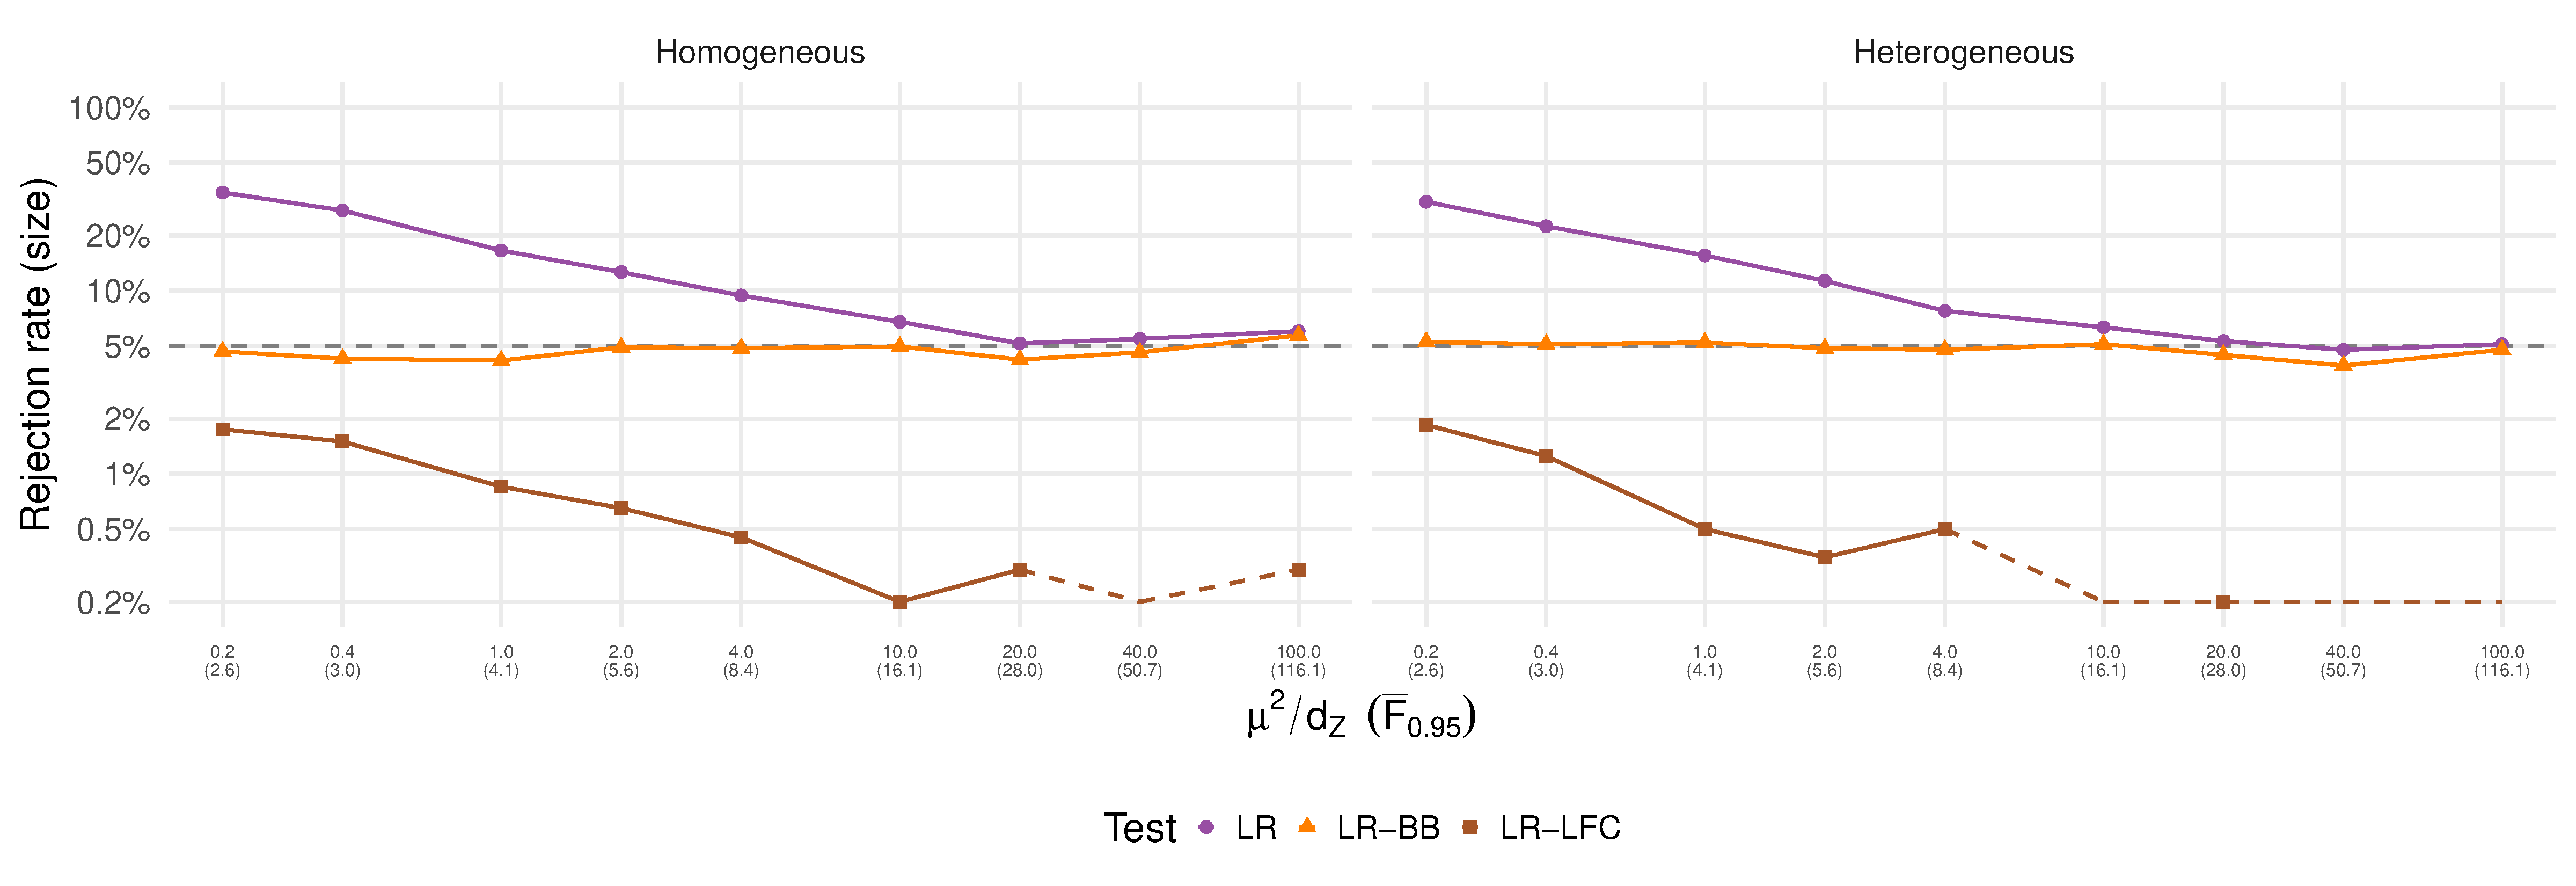
\includegraphics[width=\textwidth]{figs/inference_size_lr_dz5_rho0.999.pdf}
    \caption{\textbf{Size of the Berger-Boos corrected LR Test.} This figure plots the size of the Berger-Boos corrected LR test  for the hypothesis \(\beta=\beta_0\) when \(\beta\) is homogeneous, and when it is the TSLS/JIVE estimand (heterogeneous treatment effects), with weak instruments. The orange line shows the corrected LR test, the purple line shows the uncorrected LR test, and the brown line  shows the LFC-LR test. The y axis shows the rejection rate (size), and the x axis enumerates instrument strength.}
    \label{fig:lr-regular-asy-all}
\end{figure}


In \Cref{fig:lr-regular-asy-all-power} we plot the power of the Berger-Boos TLR test under worst-case endogeneity. We compare it to the power of the TSLS and Jaccknife IV Wald test, to obtain a notion of the degree to which the power of our test is on the level, and it is.


\begin{figure}[!htb]
    \centering
    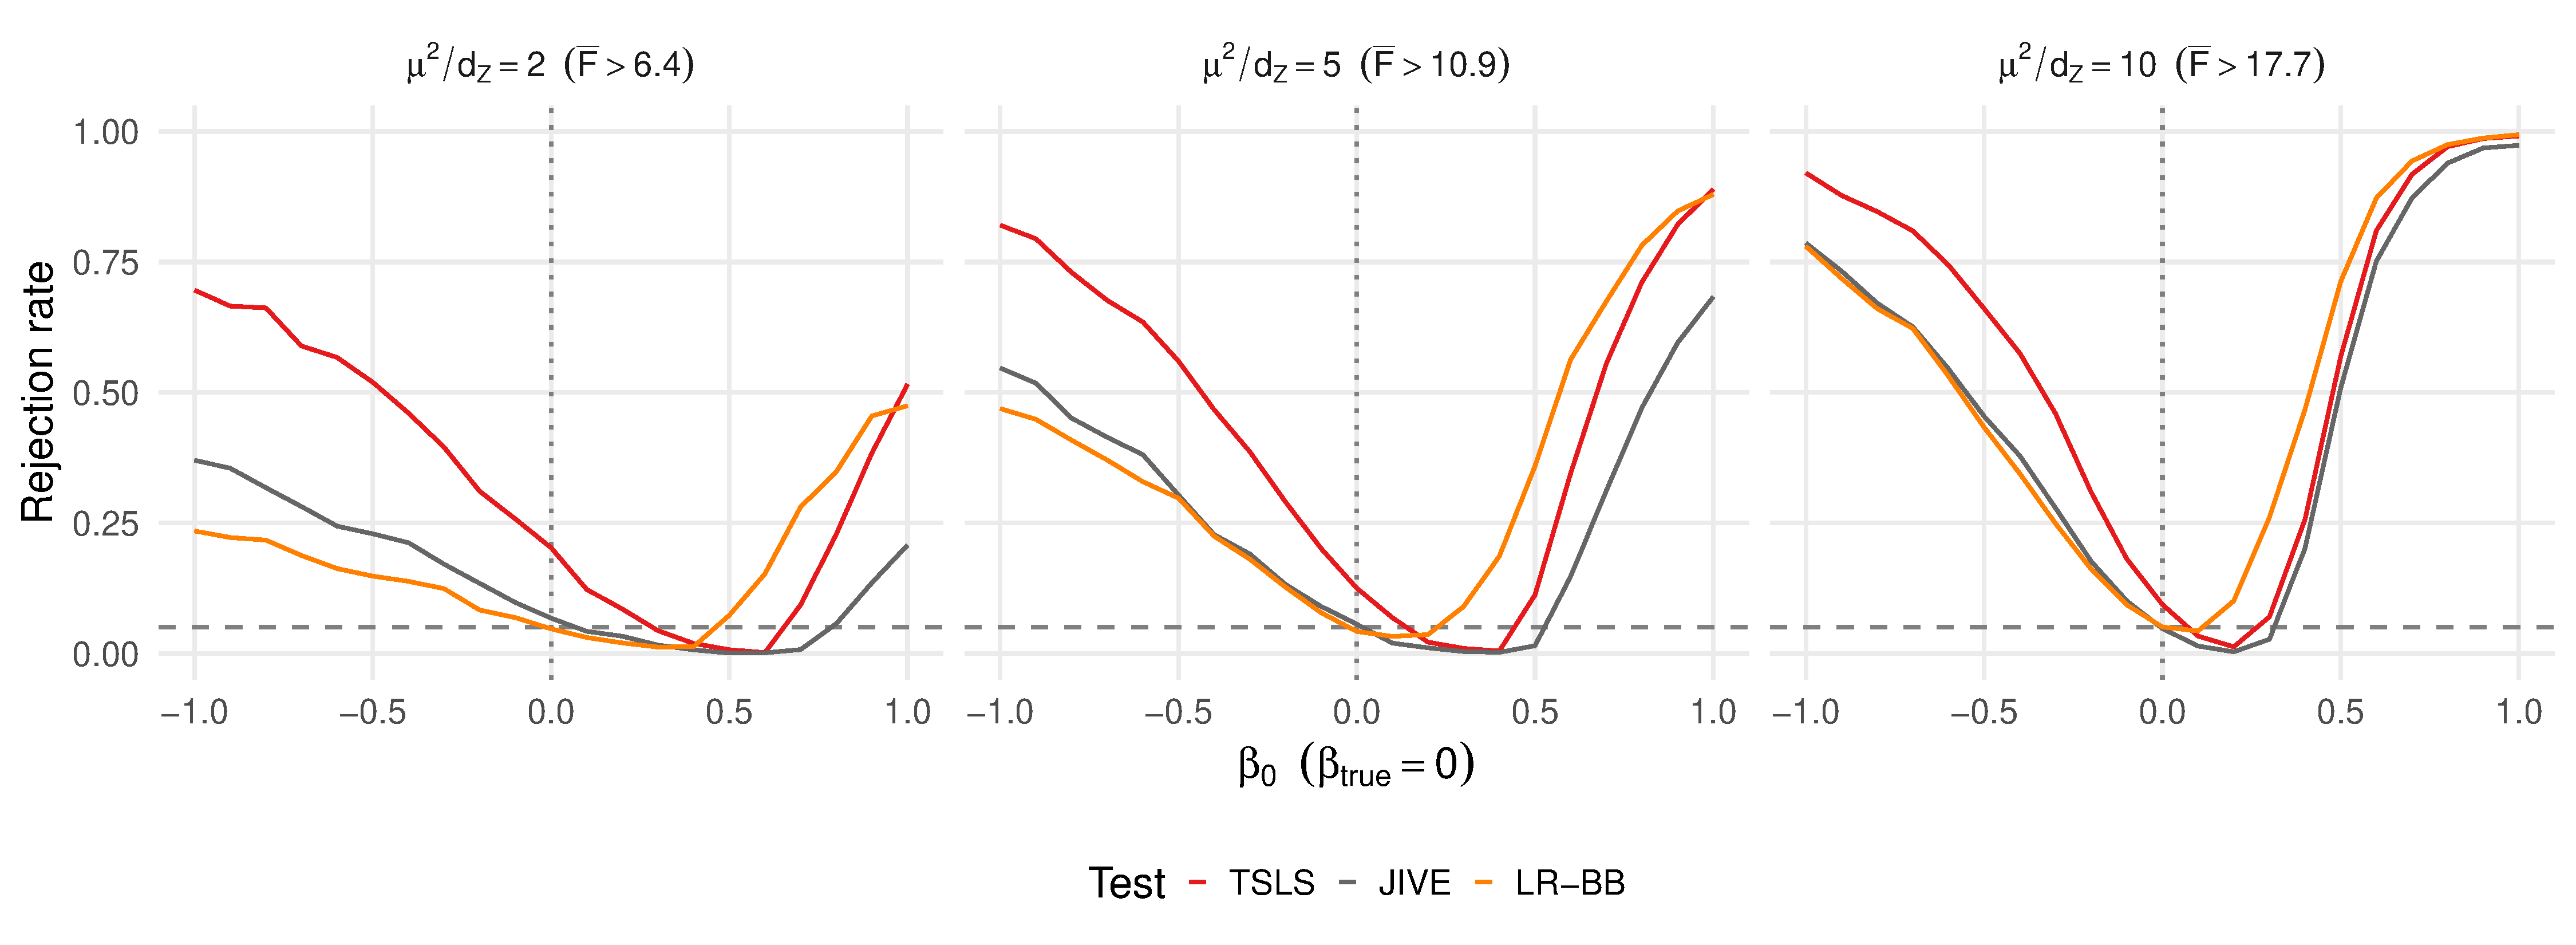
\includegraphics[width=\textwidth]{figs/inference_power_trio_dz3_rho0.999.pdf}
    \caption{\textbf{Power of the Berger-Boos corrected LR Test.} This figure plots the power against alternative of the Berger-Boos corrected LR test  for the hypothesis \(\beta=\beta_0\). The orange line shows the corrected LR test, the red line  shows the TSLS Wald test and the gray line the JIVE Wald test. The y axis shows the rejection rate, and the x axis enumerates distance from the true parameter.}
    \label{fig:lr-regular-asy-all-power}
\end{figure}

% We see that the strong-instrument test is invalid with weak instruments. We further see that the LFC TLR test is very conservative. The Berger-Boos corrected TLR test is valid and close to exact.
% \paragraph*{General Result with Continuous Treatment and Homoskedastic First Stage}





% \begin{enumerate}
%     % \item 
%     % Set up general LR problem + solution (proposition)
%     % \item 
%     % Derive strong-ID lim dist (Wilks)
    
%     \item 
%     Derive homosked continuous case + simplification
%     \item 
%     Derive binary specialized case + same simplification
%     \item 
%     Derive weak-ID lim dist -- 4dz - 1 nuisance params, no later
%     \item 
%     Set up proofs
% \end{enumerate}

% \clearpage


% \subsection{The TSLS-LR test.}

% We now turn to deriving a test that is valid under fixed \(d_Z\) and weak instruments, i.e. under the same limiting sequence considered in the previous sections of this paper.


% \paragraph*{Choice of hypothesis.}

% We are generally interested in performing inference on a weighted average of local average treatment effects (LATEs). The TSLS-JIVE estimand is one such weighted average. There are other, such as the complier-weighted average, and the complier-share squared-weighted average. Furthermore, if the analyst estimates marginal treatment effects under some linear-in-parameters model, any linear functional over this MTE curve can be retrieved as a weighted average on the TSLS-JIVE estimand form. However, for the purposes of the following, we consider the problem of imposing hypotheses on the TSLS estimand on the form:
% \begin{align}
%     \mathcal{H}_0: \beta \equiv \frac{\gamma_n'\Sigma_{ZZ}\delta_n}{\gamma_n'\Sigma_{ZZ}\gamma_n} = \beta_0
% \end{align}
% Observe that this hypothesis, or restriction, can be algebraically reformulated to a quadratic restriction on the form:
% \begin{align}
%     \mathcal{H}_0: \beta \equiv \gamma_n'\Sigma_{ZZ}(\delta_n -\beta_0\gamma_n) = 0
% \end{align}
% This will turn out to be useful in the following.

% \paragraph*{Formulating the likelihood ratio statistic.}

% Define now for convenience of notation the following two objects to be the vector of first-stage and reduced-form estimates, 
% \begin{align}
%     \tau_n \equiv 
%     \begin{bmatrix}
%         \delta_n \\
%         \gamma_n
%     \end{bmatrix} \qquad \text{and} \qquad 
%     \hat \tau \equiv 
%     \begin{bmatrix}
%         \hat \delta \\
%         \hat \gamma
%     \end{bmatrix}
% \end{align}
% and observe that we can write the asymptotic log-likelihood of \(\tau_n\) given \(\hat \tau\) as:
% \begin{align*}
%     \ell( \tau\mid \hat \tau) = L - \frac{1}{2}(\hat \tau -\tau_n)'(\Sigma/n)^{-1}(\hat \tau - \tau_n)
% \end{align*}
% The maximized unconstrained likelihood thus takes the  value of the constant \(L\).
% Multiplying by \(2\), subtracting the unconstrained from the maximized constrained log likelihood and evaluating the difference at the estimated \(\hat\Sigma\), we get the likelihood ratio statistic:
% \begin{align}
%     LR(\beta_0) \equiv \min_{\tau \in \R^{2d}}n(\hat \tau -\tau_n)'\hat \Sigma^{-1}(\hat \tau - \tau_n) \quad \text{s.t.} \quad  \gamma_n'\hat \Sigma_{ZZ}(\delta_n -\beta_0\gamma_n) = 0
% \end{align}
% This is essentially the orthogonal projection of the unconstrained maximizer onto the null manifold. In order to solve the optimization problem, we reformulate the constraint. In particular, define \(\Gamma(\beta_0)\) and \(\hat\Gamma(\beta_0)\) such that the statistic can be written as:\footnote{In particular, let 
%     \(
%     \tau_n'\,\hat\Gamma(\beta_0) \,\tau_n = 0
%     \Gamma(\beta_0) \equiv 
%     \left[\begin{smallmatrix}
%         0 & \Sigma_{ZZ} \\
%         \Sigma_{ZZ} & -2\beta_0\Sigma_{ZZ}
%     \end{smallmatrix}\right]\), and let \(\hat \Gamma(\beta_0)\) be its sample analog estimator.
% }
% \begin{align*}
% LR(\beta_0) = \min_{\tau \in \R^{2d}}\,n(\hat \tau -\tau_n)'\hat\Sigma^{-1}(\hat \tau - \tau_n) \qquad \text{s.t.} \qquad \tau_n'\,\hat\Gamma(\beta_0) \,\tau_n = 0
% \end{align*}
% Observe that \(\hat \Sigma^{-1}\) is positive definite, hence the minimiation problem is convex. The matrix \(\hat \Gamma\) is indefinite. However, by construction, it takes a saddle form.
% % are positive and negative definite, respectively. 
% The program is quadratically constrained quadratic with one constraint (QCQP-1), and is in particular an instantiation of the generalized trust region subproblem (GTRS), which is known to have a unique solution (see e.g. \citealp{sternIndefiniteTrustRegion1995}). In order to obtain this solution, we perform another re-parametrization. 
% Let \( X(\beta_0)\) denote the matrix of eigenvectors, and \( \kappa(\beta_0)\)  the vector of eigenvalues for the matrix \(\Sigma^{1/2}\,\Gamma(\beta_0)\, \Sigma^{1/2}\), and let \(\hat X(\beta_0)\) and \(\hat \kappa(\beta_0)\) denote analog estimators.
% By the nature of GTRS, \(d_Z\) eigenvalues will be positive and \(d_Z\) negative. Consider further the following change of coordinates, and let from now on dependence on \(\beta_0\) be implicit:
% \begin{align}
%     \hat W \equiv \hat X'\hat \Sigma^{-1/2}\sqrt{n}\hat \tau \qquad \text{and} \qquad  
%     w_n \equiv \hat X'\hat \Sigma^{-1/2}\sqrt{n}\tau_n
% \end{align}
% The minimization problem now simplifies as follows:
% \begin{align}
%     LR(\beta_0) = \min_{w_n \in \R^{2d}}\lVert \hat W- w_n\rVert^2 \qquad \text{s.t.} \qquad \sum_{j=1}^{2d_Z}\hat\kappa_j \,w_{n,j}^2 = 0
%     \label{eq:min-problem-re-param}
% \end{align}
% Taking the first-order conditions of the Lagrangian gives \(w_i=\hat W_i/(1+\lambda \hat \kappa_i)\), where \(\lambda\) denotes the multiplier on the constraint. Inserting back into the constraint gives the secular equation:
% \begin{align}
%     \sum_{j=1}^{2d_Z}\frac{\hat \kappa_j\hat W_{j}^2}{(1+\lambda\hat\kappa_j)^2} = 0
%     \label{eq:secular-eq}
% \end{align}
% \cite{sternIndefiniteTrustRegion1995} show that this is solved uniquely by some \(\lambda^*\) in the interval \(((\max_{j, \hat\kappa_j>0} \hat\kappa_j)^{-1},(\max_{j, \hat\kappa_j<0} |\hat\kappa_j|)^{-1})\) and its computation is numerically trivial. Inserting for the first-order condition in the minimization problem from \cref{eq:min-problem-re-param} gives the likelihood ratio statistic on semi-closed form,
% \begin{align}
%     LR(\beta_0) = \sum_{j=1}^{2d_Z}\hat W_{j}^2 \left(\frac{\lambda^*\hat \kappa_j}{1+\lambda^*\hat\kappa_j}\right)^2
% \end{align}
% where \(\lambda^*\) is the solution to the secular equation from \cref{eq:secular-eq}, and \(\{\hat \kappa_j,\hat W_j\}_{j=1}^{2d_Z}\) are observed in sample.

% \paragraph*{Evaluating the likelihood ratio statistic.}
% By \cite{wilksLargeSampleDistributionLikelihood1938} theorem (see e.g. Thm. 12.4.2(c) of \citealp{lehmannTestingStatisticalHypotheses2005}), this statistic has a chi-squared limiting distribution with one degree of freedom,
% \begin{align}
%     LR(\beta_0) \convd \mathfrak{C}^2_1
% \end{align}
% when \(n\to\infty\).
% Before we proceed to consider a weak instruments robust limiting distribution, we consider the performance of this test statistic. In \Cref{fig:lr-regular-asy} we plot the size of the test  for different \(\mu^2\) under the weak instruments approximation. We see that the LR test statistic does better than the t-test but still over-rejects for small \(\mu^2\).

% \begin{figure}[!htb]
%     \centering
%     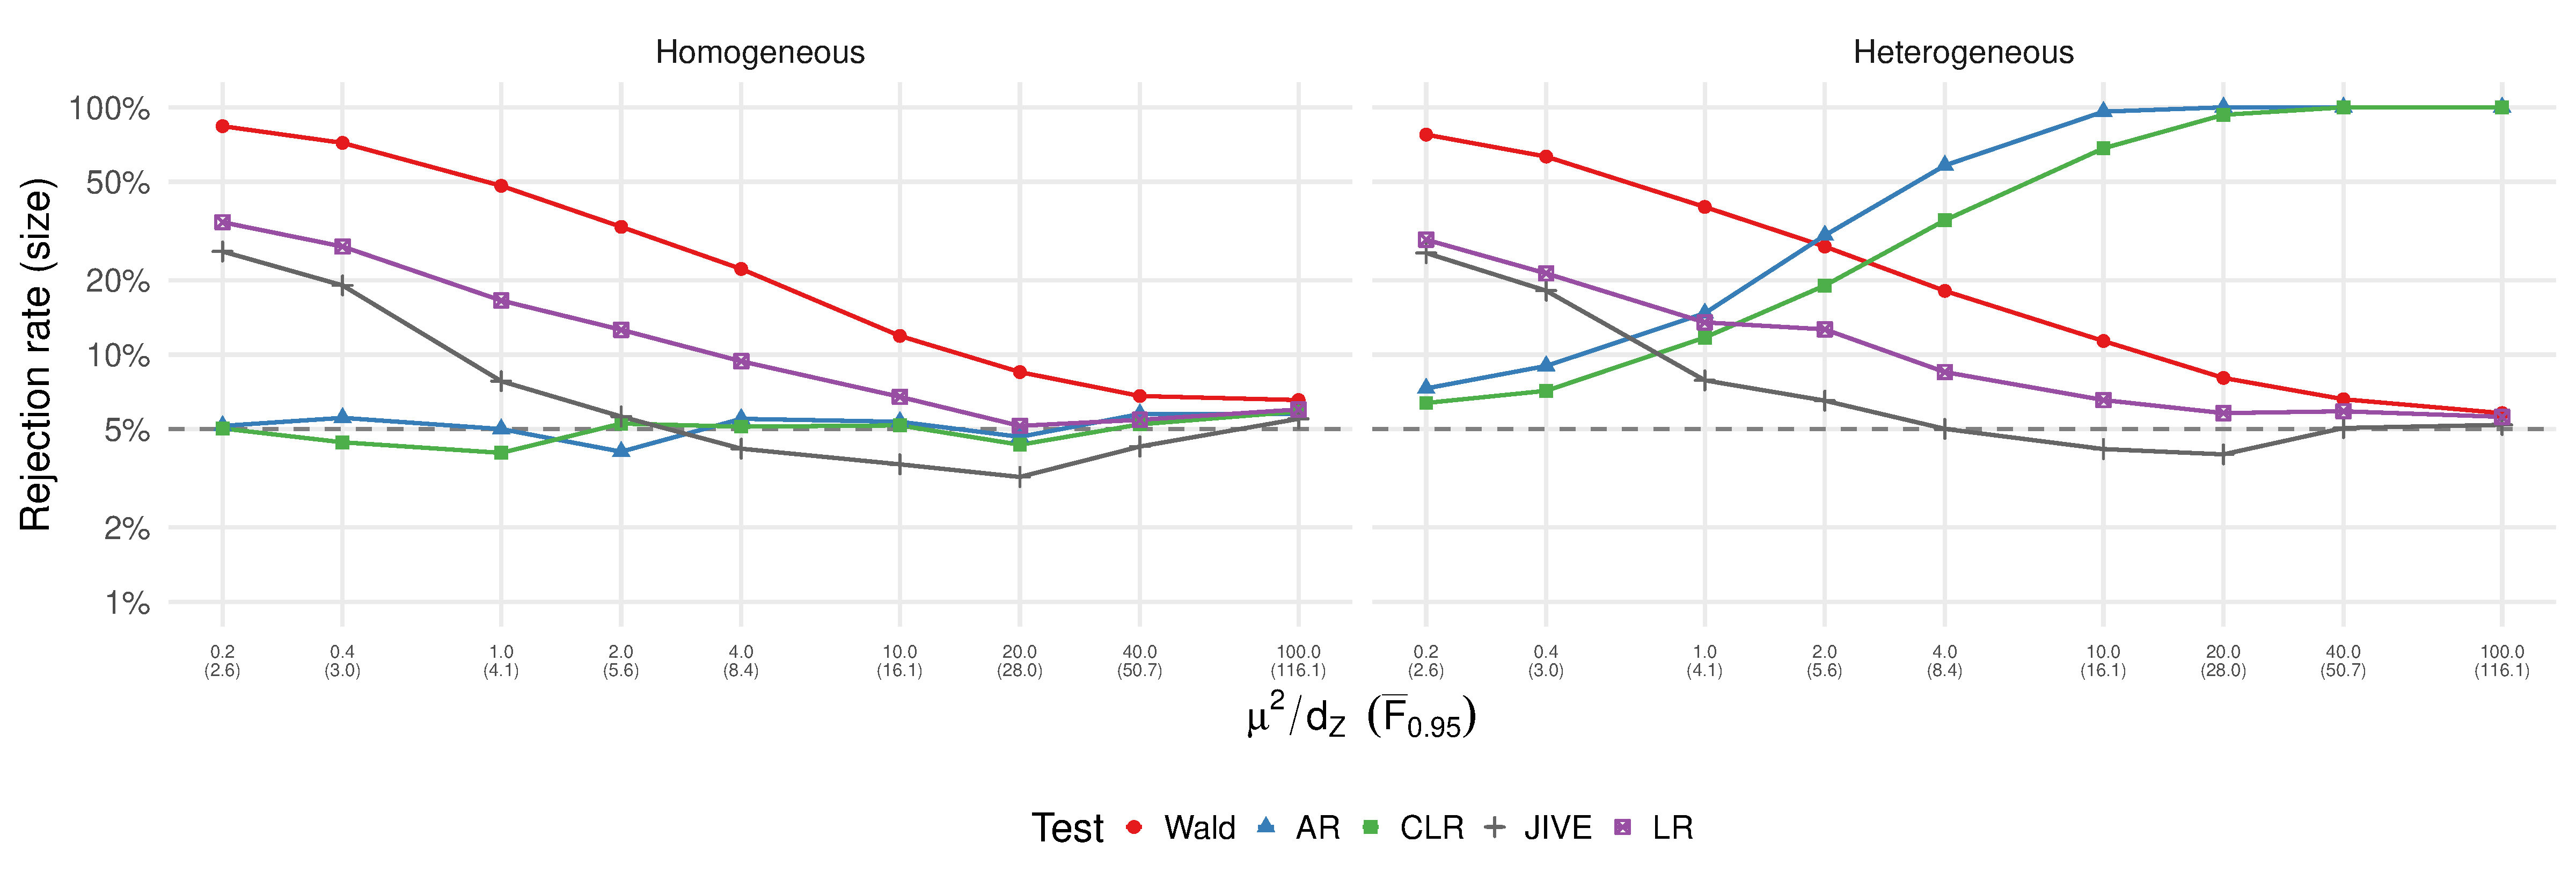
\includegraphics[width=\textwidth]{figs/inference_size_tradlr_dz5_rho0.999.pdf}
%     \caption{\textbf{Overrejection of the LR Test.} This figure plots the rate of over-rejection of the LR test for the hypothesis \(\beta=\beta_0\) when \(\beta\) is homogeneous, and when it is the TSLS/JIVE estimand (heterogeneous treatment effects), with weak instruments. The purple line shows the LR test, the red line  shows the Wald test, the blue line the AR test and the green line the CLR test. The y axis shows the rejection rate (size), and the x axis enumerates instrument strength.}
%     \label{fig:lr-regular-asy}
% \end{figure}

% The reason for this loss of validity in the weak-instruments regime is that  \cite{wilksLargeSampleDistributionLikelihood1938} theorem is only valid when the function defining the constraint has non-zero derivatives. As instruments grow weak, \(\{w_j\}_{j=1}^{d_Z}\) jointly move closer to zero, and the asymptotic approximation grows worse. It is, however, possible to derive a test that is valid under weak instruments, which we continue to consider in the following.

% \paragraph*{The likelihood-ratio statistic with weak instruments.}

% Under the weak-instrument asymptotic sequence, we have \(\sqrt{n}\gamma_n=\gamma\), and under \Cref{ass:iv} this implies \(\sqrt{n}\delta_n = \delta\).  This implies that with weak instruments, we further have 
% \begin{align*}
%     \hat W \convd W \sim \mathfrak{N}(w,\boldsymbol{\iota}_{d_Z}) 
%     \qquad \text{where} \qquad 
%     \sum_{j=1}^{2d_Z}\kappa_j w_j = 0
% \end{align*}
% for some \(2d_Z\)-dimensional vectors \((\kappa,w)\), where \(w\equiv\sqrt{n}w_n\) along the weak instruments asymptotic sequence.
% It further follows that the LR statistic has limiting distribution
% \begin{align}
%     LR(\beta_0) \convd \sum_{j=1}^{2d_Z}  W_j^2\left(\frac{\lambda^*  \kappa_j}{1+\lambda^* \kappa_j}\right)^2
% \end{align}
% Without any further structure, this problem has \(4d_Z-1\) nuisance parameters. While we have a consistent estimator for \(\kappa\), we do not for \(w\), and in any case, it is not trivial to search over the whole nuisance space even with a sufficient statistic for \(w\).

% \paragraph*{Simplification with binary treatment.}

% We now return our focus to the binary treatment and saturated instrument setting of the previous sections.
% Assume eigenvalues of \(\Sigma^{1/2}\Gamma(\beta_0)\Sigma^{1/2}\) exist in pairs of one positive and one negative eigenvalue. Let these eigenvalues be denoted \(\kappa^{(k)}_+\) and \(\kappa^{(k)}_-\), \(k=1,\ldots,d_Z\). By the structure of the binary-saturated design, we can thus state a conjecture.

% \begin{conjecture}\label{conj:binary-treat-limit}
%     With binary treatment, along the weak-instrument asymptotic sequence, we have 
%     \begin{align}
%         \kappa^{(k)}_{{\pm}} \xrightarrow{n\to\infty} \kappa^*_{\pm}
%     \end{align}
%     In particular, we also have
% \begin{align}
%     \varrho^{(k)} \equiv \frac{\lvert\kappa^{(k)}_{{-}}\rvert}{\kappa^{(k)}_{{+}}} \xrightarrow{n\to\infty}
%      \frac{\lvert\kappa^*_{{-}}\rvert}{\kappa^*_{{+}}} \equiv \varrho^*
% \end{align}
% \end{conjecture}
% \begin{remark}
%     This follows from the same logic that simplifies the limiting distribution of the TSLS and JIVE estimators with weak instruments. We might not need it, if Sattherwaithe approximation goes through, so let's wait to prove it.
% \end{remark}
% \noindent
% Observe that under \Cref{conj:binary-treat-limit}, we can write the secular equation along the weak instruments limiting sequence as:
% \begin{align*}
%     \frac{ \kappa_+^* }{(1+\lambda^*\kappa^*_+)^2}\sum_{\kappa_j>0}W_{j}^2 
%     -\frac{ \lvert\kappa_-^*\rvert }{(1-\lambda^*\lvert\kappa_-^*\rvert)^2}\sum_{\kappa_j<0}W_{j}^2  = 0
% \end{align*}
% Observe now that
% \begin{align}
%     Q_+ \equiv \sum_{\kappa_j>0}W_j^2 \sim \mathfrak{C}^2_{d_Z}(\xi_+)
%     \qquad \text{and}
%     \qquad 
%     Q_- \equiv \sum_{\kappa_j<0}W_j^2 \sim \mathfrak{C}^2_{d_Z}(\xi_-)
% \end{align}
% where \(Q_+,Q_-\) are independent, and under the null we have along the asymptotic sequence, where \(\sqrt{n}w_n=w\), that:
% \begin{align*}
%     \sum_{j=1}^{2d_Z}\kappa_jw_j^2 = 0
%     \iff
%         \lvert\kappa_-\rvert\sum_{\kappa_j<0}w_j^2 = \kappa_+\sum_{\kappa_j>0}w_j^2
% \end{align*}
% and by the properties of non-central chi-squared distributions, this implies \(\varrho^*\xi_- = \xi_+ \equiv \xi\).
% The secular equation thus simplifies as:
% \begin{align*}
%     \frac{ Q_+ }{(1+\lambda^*\kappa^*_+)^2}
%      = \frac{ \varrho^* Q_- }{(1-\lambda^*\lvert\kappa_-^*\rvert)^2} 
% \end{align*}
% Taking the root and solving for \(\lambda^*\kappa_+^*\), we obtain:
% \begin{align*}
% \lambda^*\kappa_+^* = 
%     \frac{ \sqrt{Q_+}-\sqrt{\varrho^*Q_-}}{\varrho^*\sqrt{Q_+} + \sqrt{\varrho^*Q_-}}
%     \label{eq:secular-simplific}
% \end{align*}
% Under \Cref{conj:binary-treat-limit} the LR statistic obtains:
% \begin{align*}
%     LR(\beta_0) \convd 
%      \left(\frac{\lambda^*  \kappa^*_+}{1+\lambda^* \kappa^*_+}\right)^2Q_++\left(\frac{\lambda^*  \kappa^*_-}{1+\lambda^* \kappa^*_-}\right)^2Q_- 
% \end{align*}
% Inserting for \cref{eq:secular-simplific} in this limit, we obtain:
% \begin{align*}
%     LR(\beta_0) \convd 
%      \left(\frac{\sqrt{Q_+}-\sqrt{\varrho^* Q_-}}{\left(1+\varrho^*\right) \sqrt{Q_+}}\right)^2 Q_+
%      +\left(\frac{\varrho^*\left(\sqrt{Q_+}-\sqrt{\varrho^* Q_-}\right)}{\left(1+\varrho^*\right) \sqrt{\varrho^* Q_-}}\right)^2 Q_-
% \end{align*}
% This simplifies to:
% \begin{align}
%     LR(\beta_0) \convd 
%     \frac{\left(\sqrt{Q_+}-\sqrt{\varrho^* Q_-}\right)^2}{1+\varrho^*}
% \end{align}
% where \(Q_+ \sim \mathfrak{C}^2_{d_Z}(\xi)\) and \(Q_- \sim \mathfrak{C}^2_{d_Z}(\xi/\varrho^*)\).
% Our limiting distribution is thus simplified to a known distribution with two nuisance parameters, \(\varrho^*\) and \(\xi\). Observe that \(\varrho^*\) can be consistently estimated. Let the estimator be denoted \(\hat \varrho\). For every \(\hat \varrho\), we can thus compute the least favorable (LFC) limiting distribution to obtain uniformly valid quantiles.

% \paragraph*{A Berger \& Boos-corrected likelihood ratio test.}
% The LFC limiting distribution ends up being very conservative. This is driven by boundary values for \(\xi\).
% Note however that we have the summary statistic
% \begin{align*}
%     \hat S \equiv \sum_{\hat\kappa_j>0}\hat W_j^2 + \sum_{\hat\kappa_j<0}\hat W_j^2 \convd
%     Q_+ + Q_- \sim \mathfrak{C}^2_{2d_Z}\left(\xi\left(1+\frac{1}{\varrho^*}\right)\right)
% \end{align*}
% This can be inverted to form a CI for \(\xi\) at some level \(\alpha_1\). Denote this CI \(\bar \Xi_{1-\alpha_1}\). Following \cite{bergerValuesMaximizedConfidence1994}, we can take the least favorable \(\xi\) over this interval at level \(\alpha_1\), insert for this and perform the likelihood ratio test at level \(\alpha_2\). The test procedure then has level
% \begin{align*}
%     P(LR(\beta_0) \geq \max_{\xi \in \bar \Xi_{1-\alpha_1}} c_{\hat \rho}(\xi) ) \to \alpha_1 + \alpha_2 = \alpha
% \end{align*}
% This test will have level \(\alpha\). It turns out that the worst-case quantiles are not very sensitive to the choice of \(\alpha_1\). Hence we can chose \(\alpha_1\) almost arbitrarily small and still obtain substantial power gains. In the following we set \(\alpha_1=10^{-5}\). We call this the Berger-Boos LR test.

% In \Cref{fig:lr-regular-asy-all} we show that both the LR-LFC and the Berger-Boos LR test is consistent in level under the weak instruments sequence. The LR-LFC test is very conservative. However, the LR-BB test does much better, essentially being worst-case exact.




% \paragraph*{Inference on MTE Functionals.}


% \begin{conjecture}
%     This extends to any weighting scheme, we can replace \(\Sigma_{ZZ}\) with any weighting matrix \(\Omega\). Since any linear functional of an MTE curve specified using a linear-in-parameters specification can be computed as a \(\gamma_n\)-weighted average of \(\delta_n\), we can perform weak-instrument robust inference on any such linear functional, including the ATE, ATT, ATU or policy relevant treatment effect (PRTE).
% \end{conjecture}

% TBC.
% Having derived asymptotic approximations to the distribution of the TSLS and JIVE estimators with weak instruments, we can also derive their bias. We do this in the following.

% \paragraph*{The generalized bias of TSLS.}
% Given that the asymptotic approximation to the distribution of the TSLS estimator with binary treatment takes the same form as its distribution under homoskedasticity, there exist analytic results for its bias due to \cite{richardsonNoteComparisonOrdinary1971}.  With \(d_Z\geq 2\) instruments, the bias is defined as its expectation. With one instrument, it is possible to approximate an intuitive notion of bias as its principal value, as shown by \cite{mogstadBiasIVOne2026}, who also derive a closed form in this case and show that it is identical to the formula given by Richardson and Wu. We record it as a lemma.
% \begin{lemmap}{GEN-TSLS}[Bias of the TSLS Estimator]\label{lem:gen-tsls}
% With binary treatment, the bias of the TSLS estimator is given as follows.
% \begin{align}
%     b_{d_Z}^{\text{TSLS}}(\mu^2,\omega) = \omega \cdot \exp\left(-\frac{\mu^2}{2}\right) {}_1F_1 \left(\frac{d_Z}{2}-1,\frac{d_Z}{2},\frac{\mu^2}{2}\right)
% \end{align}
%     where \({}_1F_1(\cdot,\cdot,\cdot)\) is the confluent hypergeometric function of the first kind.
% \end{lemmap}
% \begin{proof}
%     See \cite{hardingFiniteSampleBIAS2016} and \cite{mogstadBiasIVOne2026}.
% \end{proof}

% \paragraph*{The generalized bias of JIVE.}
% The JIVE estimator does not possess well-defined moments. However, \cite{mogstadBiasIVOne2026} define a notion of bias that is well-defined for heavy-tailed distributions. This notion of bias is called trimmed bias, and captures the direction and magnitude of a typical error, when a share \((1-\lambda)\) of estimation errors \(\hat B - \beta\) are considered typical and a share \(\lambda\in(0,1)\) are considered atypical. They show that for distributions with symmetric tails, it is possible to approximate the bias when all errors are considered typical by considering the \emph{Cauchy principal value} of the distribution of estimation errors. This notion of bias is called \emph{generalized bias}. In \Cref{fig:trimmed-mean-gen-bias-jive} we plot the trimmed bias of the JIVE estimator with \(d_Z=5\) for some shares \(\lambda\). The figure shows that the trimmed bias settles down as \(\lambda\to 0\). This indicates symmetric tails. We record this observation and the generalized bias of the JIVE estimator formally as a proposition.


% \begin{figure}[!htb]
%     \centering
    
%    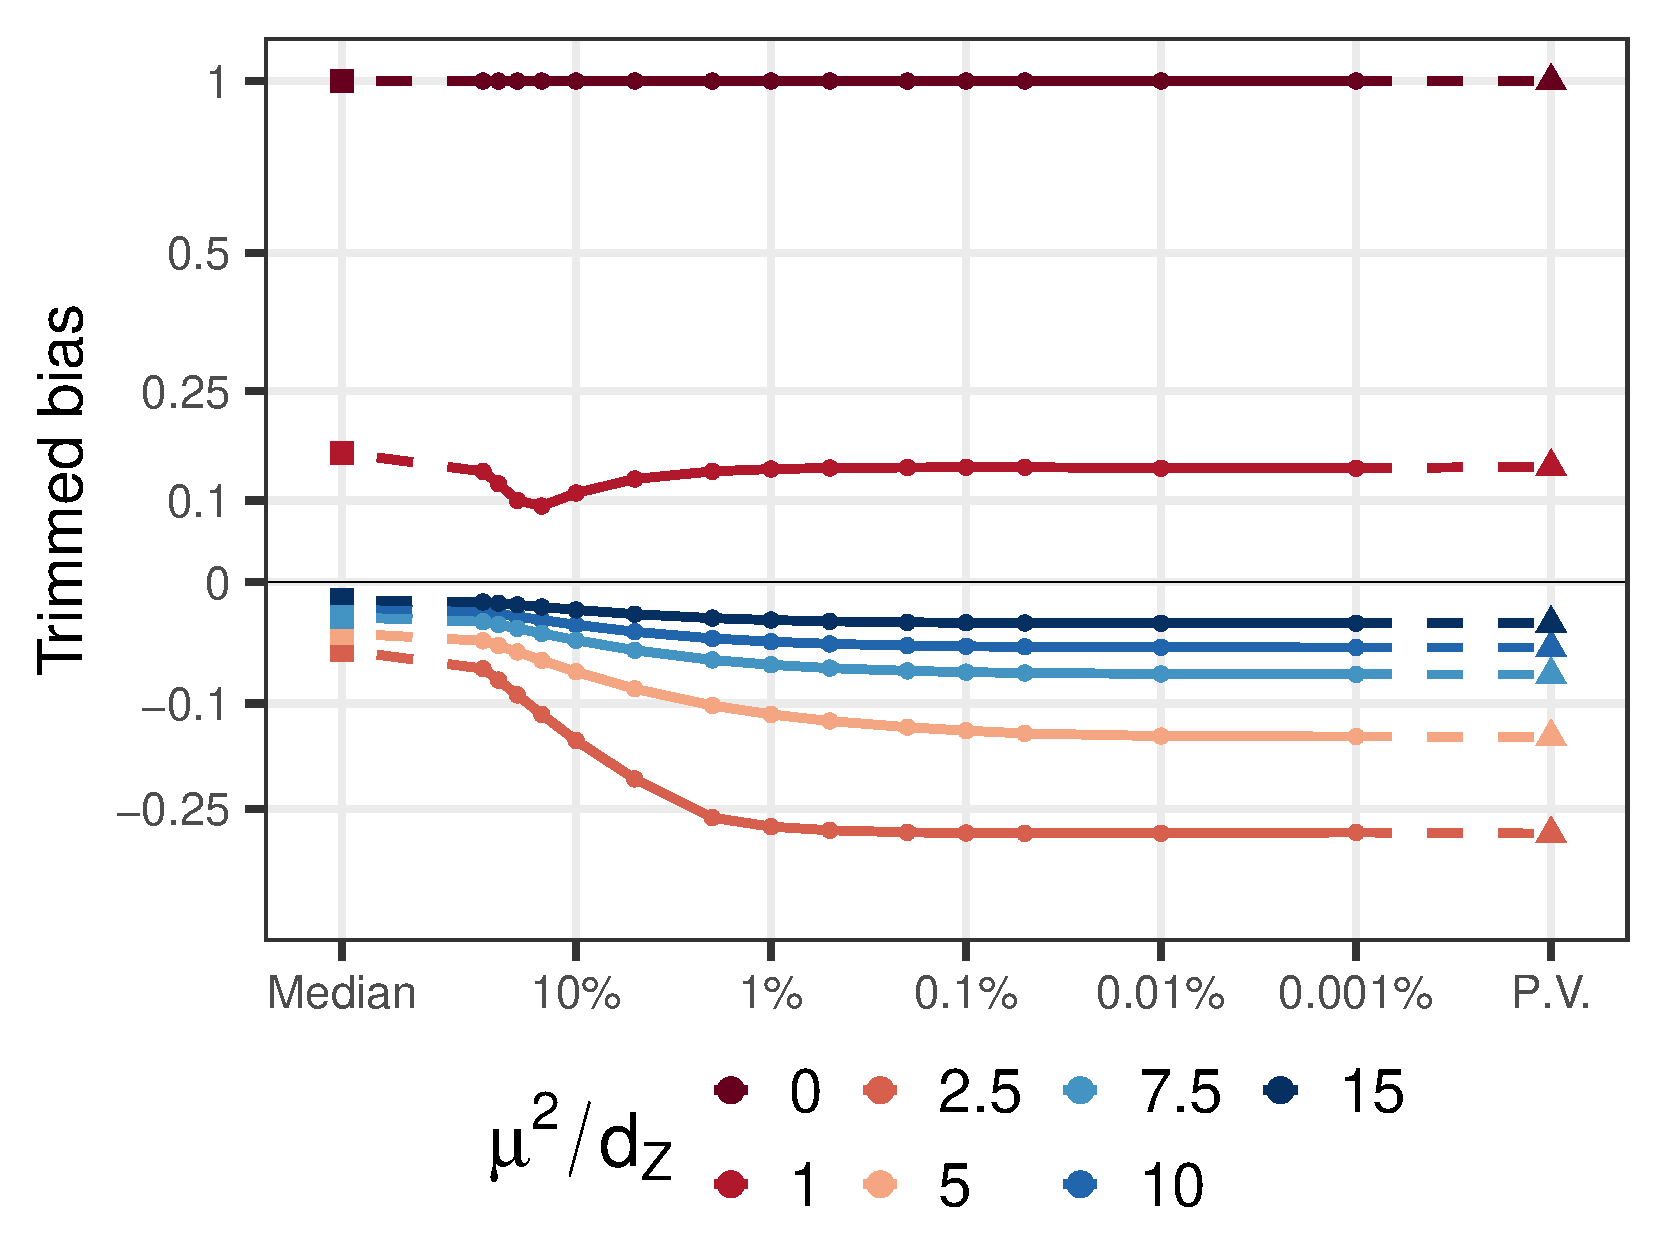
\includegraphics[width=0.75\textwidth ]{figs/limit_trimbias_jive_dz5.pdf}

%     \caption{\textbf{Trimmed bias for different \(\lambda\).} This figure shows how the trimmed bias of the IV estimator differs for different \(\lambda\). The trimmed bias is shown for a selection of  \(\mu^2\), relative to \(\omega\). The limit as \(\lambda\uparrow 1\) and \(\lambda\downarrow 0\) are indicated as ``Median'' and ``P.V.'', respectively. 
%       }
%       \label{fig:trimmed-mean-gen-bias-jive}
% \end{figure}

% \begin{propositionp}{GEN-JIVE}[Cauchy Principal Value of the JIVE Estimator]\label{prop:gen-jive}
% The asymptotic distribution of the Jackknife IV estimator has symmetric tails.
% With binary treatment, the generalized bias of the JIVE estimator is given as follows.
% \begin{align}
%     b_{d_Z}^{\textup{JIVE}}(\mu^2,\omega) = \omega \left(1 - \int_0^\infty \kappa\!\left(\sqrt{\mu^2},\; w - d_Z\right) f_{d_Z - 1}(w)\, dw \right)
% \end{align}
% where $f_{d_Z-1}(w)$ is the $\mathfrak{C}^2_{d_Z-1}$ density and $\kappa$ is given as
% \begin{align}\label{eq:cpv-kernel}
%     \kappa(m, \delta) =
%     \begin{dcases}
%         \displaystyle\frac{m}{\sqrt{2}} \left[ D\!\left(\frac{m - \sqrt{-\delta}}{\sqrt{2}}\right) + D\!\left(\frac{m + \sqrt{-\delta}}{\sqrt{2}}\right) \right] & \text{if } \delta \leq 0, \\[8pt]
%         \displaystyle\int_{-\infty}^{\infty} \frac{m\, t}{t^2 + \delta}\; \varphi(t - m)\, dt & \text{if } \delta > 0,
%     \end{dcases}
% \end{align}
% with $D(x) = e^{-x^2}\int_0^x e^{t^2}\,dt$ the Dawson function and $\varphi$ the standard normal density.
% \end{propositionp}
% \begin{proof}
% See Appendix \ref{appx:proof-gen-jive}.
% \end{proof}
% \noindent
% While the bias of the JIVE estimator does not have a closed-form solution, and also not a solution in terms of known analytic functions, it can be computed at low cost with known numerical methods.

% In \Cref{fig:bias-jive-tsls}, we plot the generalized bias of the TSLS and JIVE estimators with binary treatment for a range of different number of instruments and concentration parameters, \(\mu^2\). 
% \begin{figure}[!b]
%     \centering
%     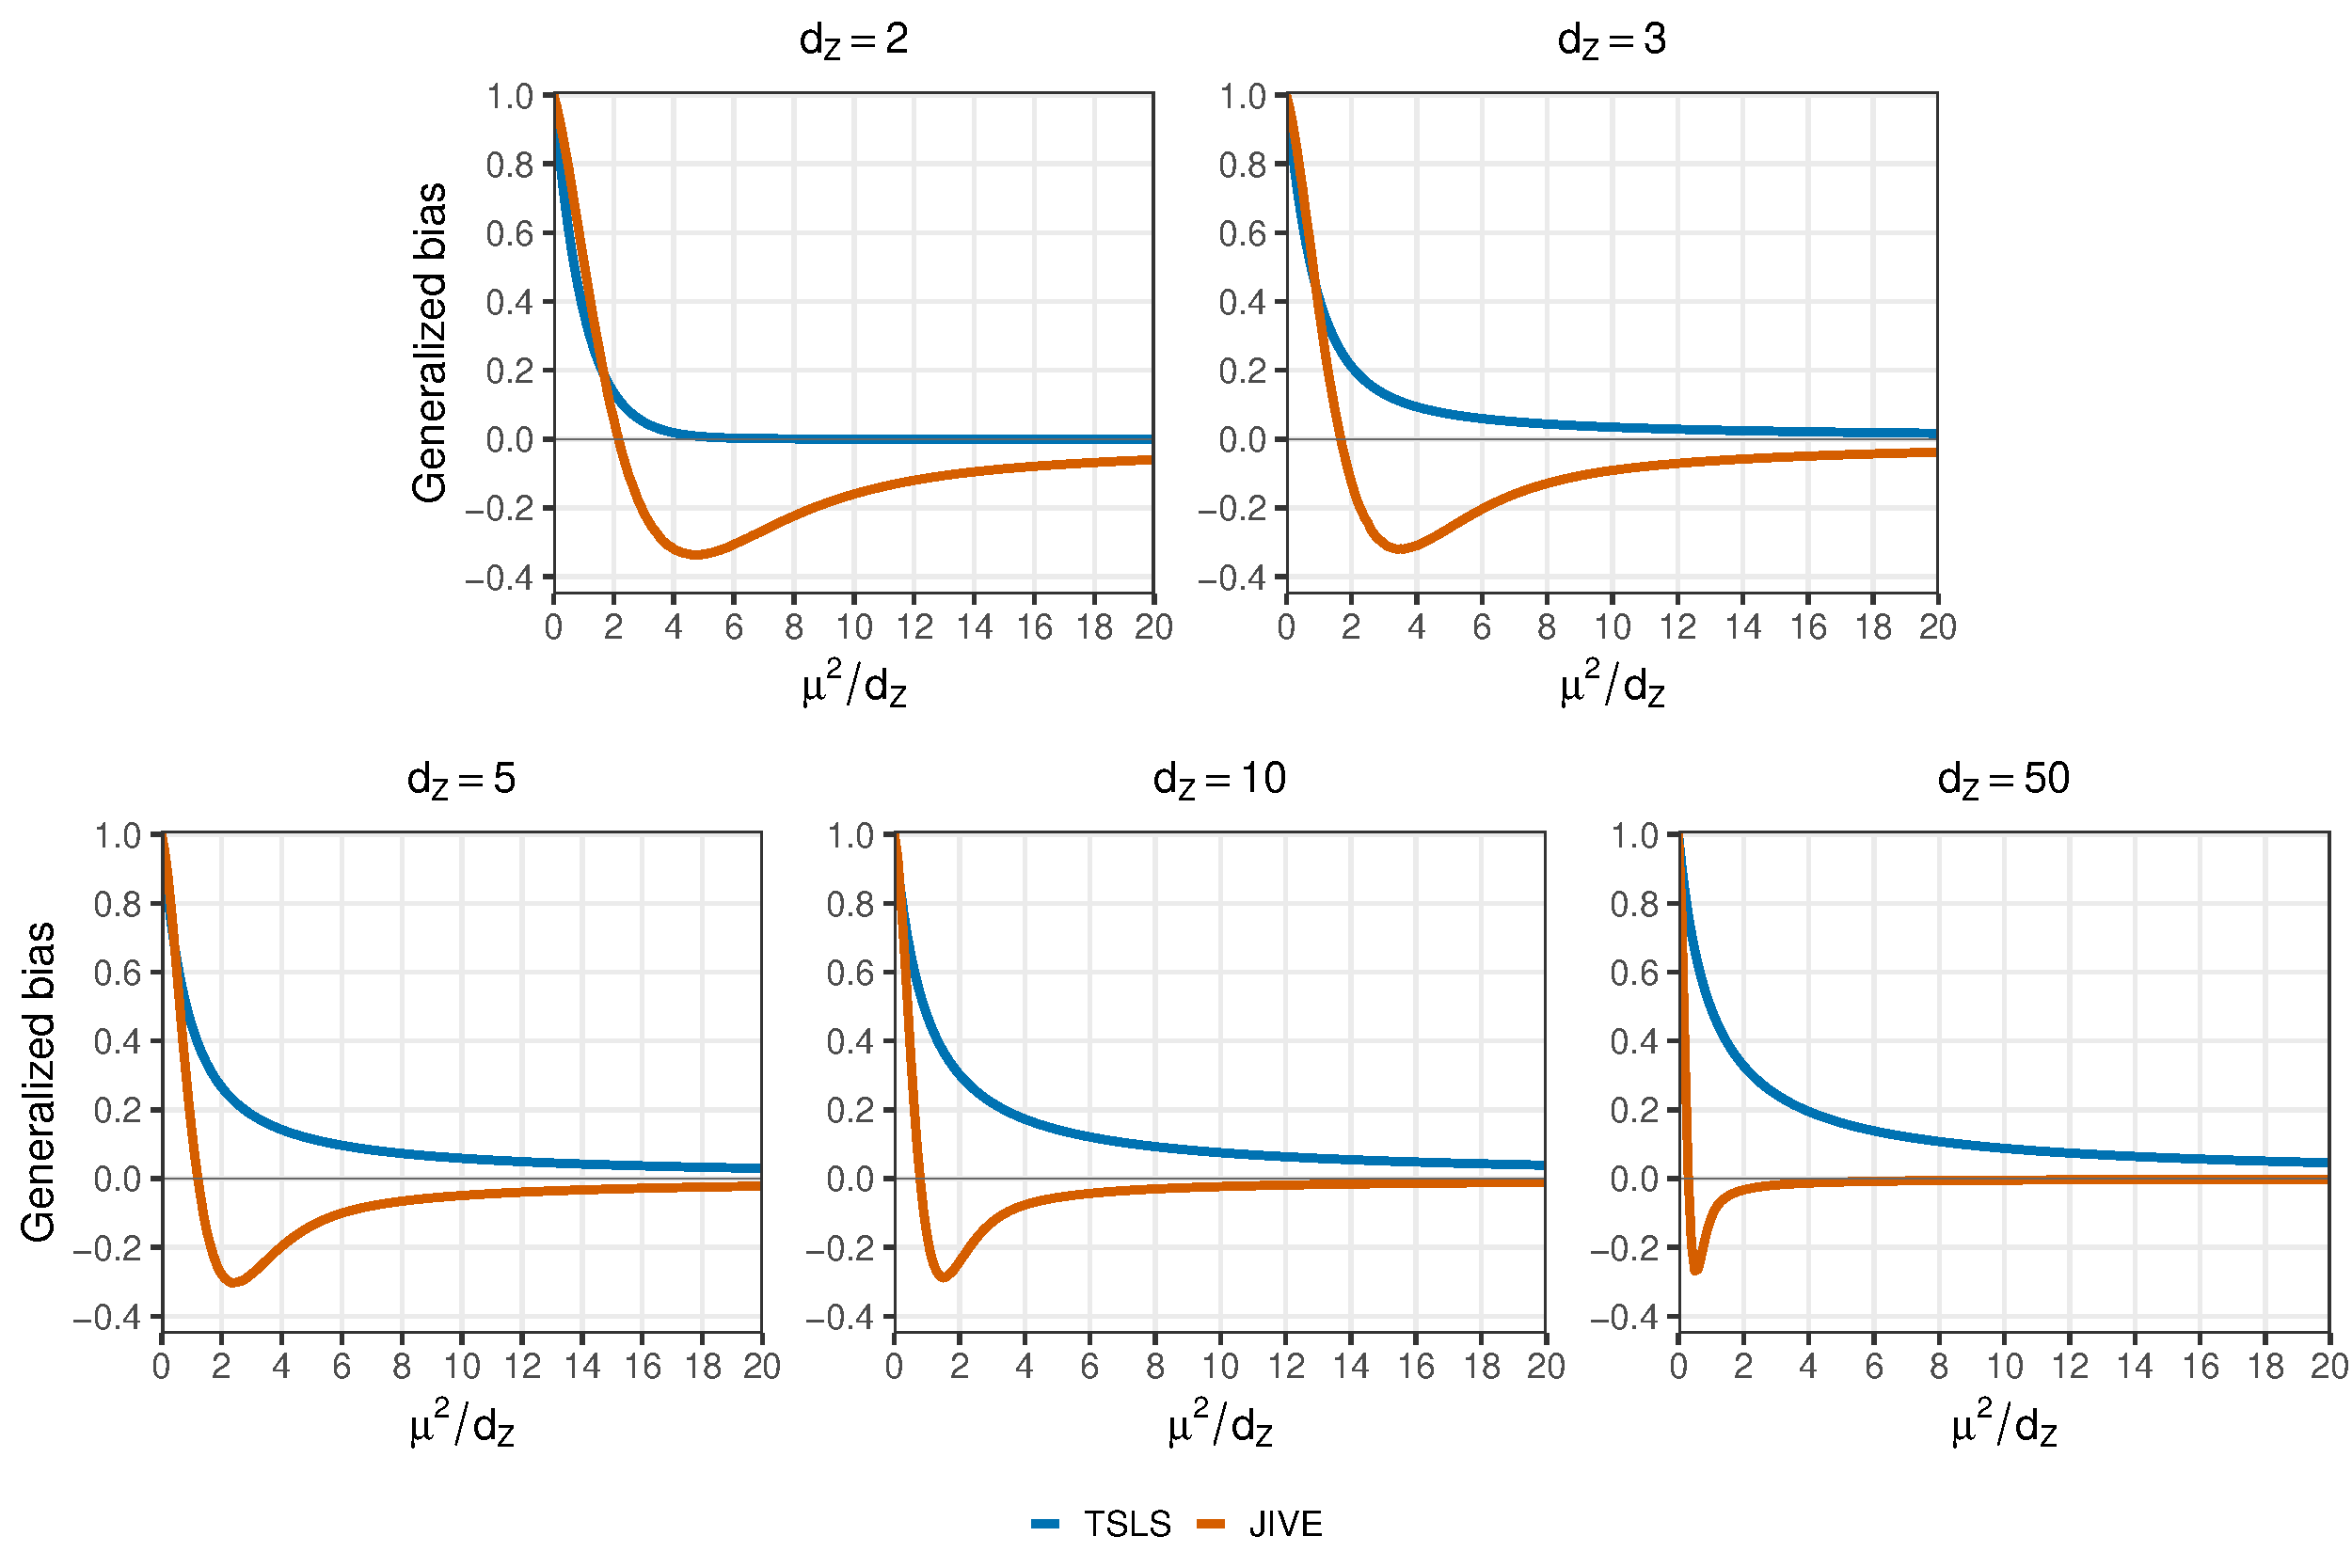
\includegraphics[width=\textwidth]{figs/limit_bias_tsls_jive_by_dz.pdf}
%     \caption{\textbf{Generalized Bias of the TSLS and JIVE Estimators.} This figure shows 
%     the generalized bias of the TSLS and JIVE estimators for different numbers of instruments, \(d_Z\) and different values of the concentration parameter. Bias is shown as a function of \(\mu^2/d_Z\) which can be thought of as the average concentration of each instrument. Bias is shown relative to \(\omega\). 
%       }
%     \label{fig:bias-jive-tsls}
% \end{figure}
% The x axis is enumerated in terms of the average concentration per instrument, \(\mu^2/d_Z\). Three observations are apparent. First, the bias of the TSLS estimator for a fixed instrument strength, \(\mu^2\), grows as the number of instruments grow, \(d_Z\to \infty\). This is consistent with the result from \cite{bekkerAlternativeApproximationsDistributions1994} that the TSLS has a \emph{many-instruments} bias. Second, the bias of the JIVE estimator, as a function of \(\mu^2/d_Z\), decreases as \(d_Z\to\infty\). This is consistent with the results from \cite{chaoAsymptoticDistributionJive2012} that the JIVE estimator is many-instruments unbiased, but that it might  have \emph{many-weak-instruments} bias. The third observation is that for \(d_Z\geq 2\), the bias of the two estimators are signed in different directions relative to the asymptotic benchmark, \(\omega\).

% The fact that the two estimators have opposite-signed bias for \(d_Z\geq 2\) indicates that some combination of the two estimators might reduce overall bias. We turn to deriving this estimator in the following.

% \paragraph*{Minimizing the bias of TSLS and JIVE.}

% While the bias of the TSLS and JIVE estimator are opposite-signed, they are not symmetric around zero. Hence, it is not possible to bring the bias to zero with a convex combination. However, it will turn out to be possible to reduce bias substantially by considering a positively weighted average of the two estimators, in the case of \(d_Z\geq 2\) instruments.

% How do we decide which weighted average to consider? A natural candidate is to make an attempt at cancelling the first-order bias as \(\mu^2\to \infty\). This is exactly the notion of bias developed by \cite{nagarBiasMomentMatrix1959}, and captured by what is often referred to as \emph{Nagar bias}. As a first step, thus, we record the Nagar bias of the TSLS and JIVE estimators as a lemma.

%   \begin{lemmap}{NAGAR}\label{lem:nagar}
%   Let Nagar bias be defined as in \cite{nagarBiasMomentMatrix1959}.
%   The TSLS and JIVE estimators have Nagar bias given as follows.

%   \begin{align}\label{eq:nagar}
%   \ddot b_{d_Z}^{\textup{TSLS}}(\mu^2, \omega) = \omega \cdot\frac{(d_Z - 2)}{\mu^2}
%   \qquad\qquad
%   \ddot b_{d_Z}^{\textup{JIVE}}(\mu^2, \omega) = -\omega \cdot\frac{2}{\mu^2}.
%   \end{align}
%   \end{lemmap}
%   \begin{proof}
%       See Appendix~\ref{appx:proof-nagar}.
%   \end{proof}


% \noindent 
% Now, we can consider whether it is possible to find an estimator that is Nagar unbiased, and study its properties. It turns out that this is possible. We record the result as a proposition.


%   \begin{propositionp}{COMB}\label{prop:comb}
%   Define the following estimator as the convex combination of the TSLS and JIVE estimators for \(d_Z\geq 2\).
%   \begin{align}\label{eq:comb-def}
%   \hat{B}_{\textup{COMB}} &\equiv \frac{2}{d_Z}\, \hat{B}_{\textup{TSLS}} + \frac{d_Z-2}{d_Z}\, \hat{B}_{\textup{JIVE}}
%   \end{align}
%     This estimator is Nagar unbiased.  
%   \end{propositionp}
%   \begin{proof}
%   See Appendix~\ref{appx:proof-combo}.
%   \end{proof}

% \noindent
% Having derived the Nagar unbiased combined estimator, it is of interest to compare its generalized bias to the bias of the TSLS and Jackknife IV estimator. 
% In \Cref{fig:bias-jive-tsls-combined}, we plot the bias of the combined TSLS-JIVE estimator. We see that the bias of the estimator is between the bias of JIVE and TSLS in all cases, and further that it is smaller in absolute value. The bias reduction is most substantial for \(d_Z\leq 10\), and by \(d_Z=50\), the estimator essentially has the same bias as the JIVE estimator. This is not strange, as the weight on the TSLS estimator is at this point only \(1/25\), whereas \(24/25\) of the weight is put on the JIVE estimator.

% \begin{figure}[!htb]
%     \centering
%     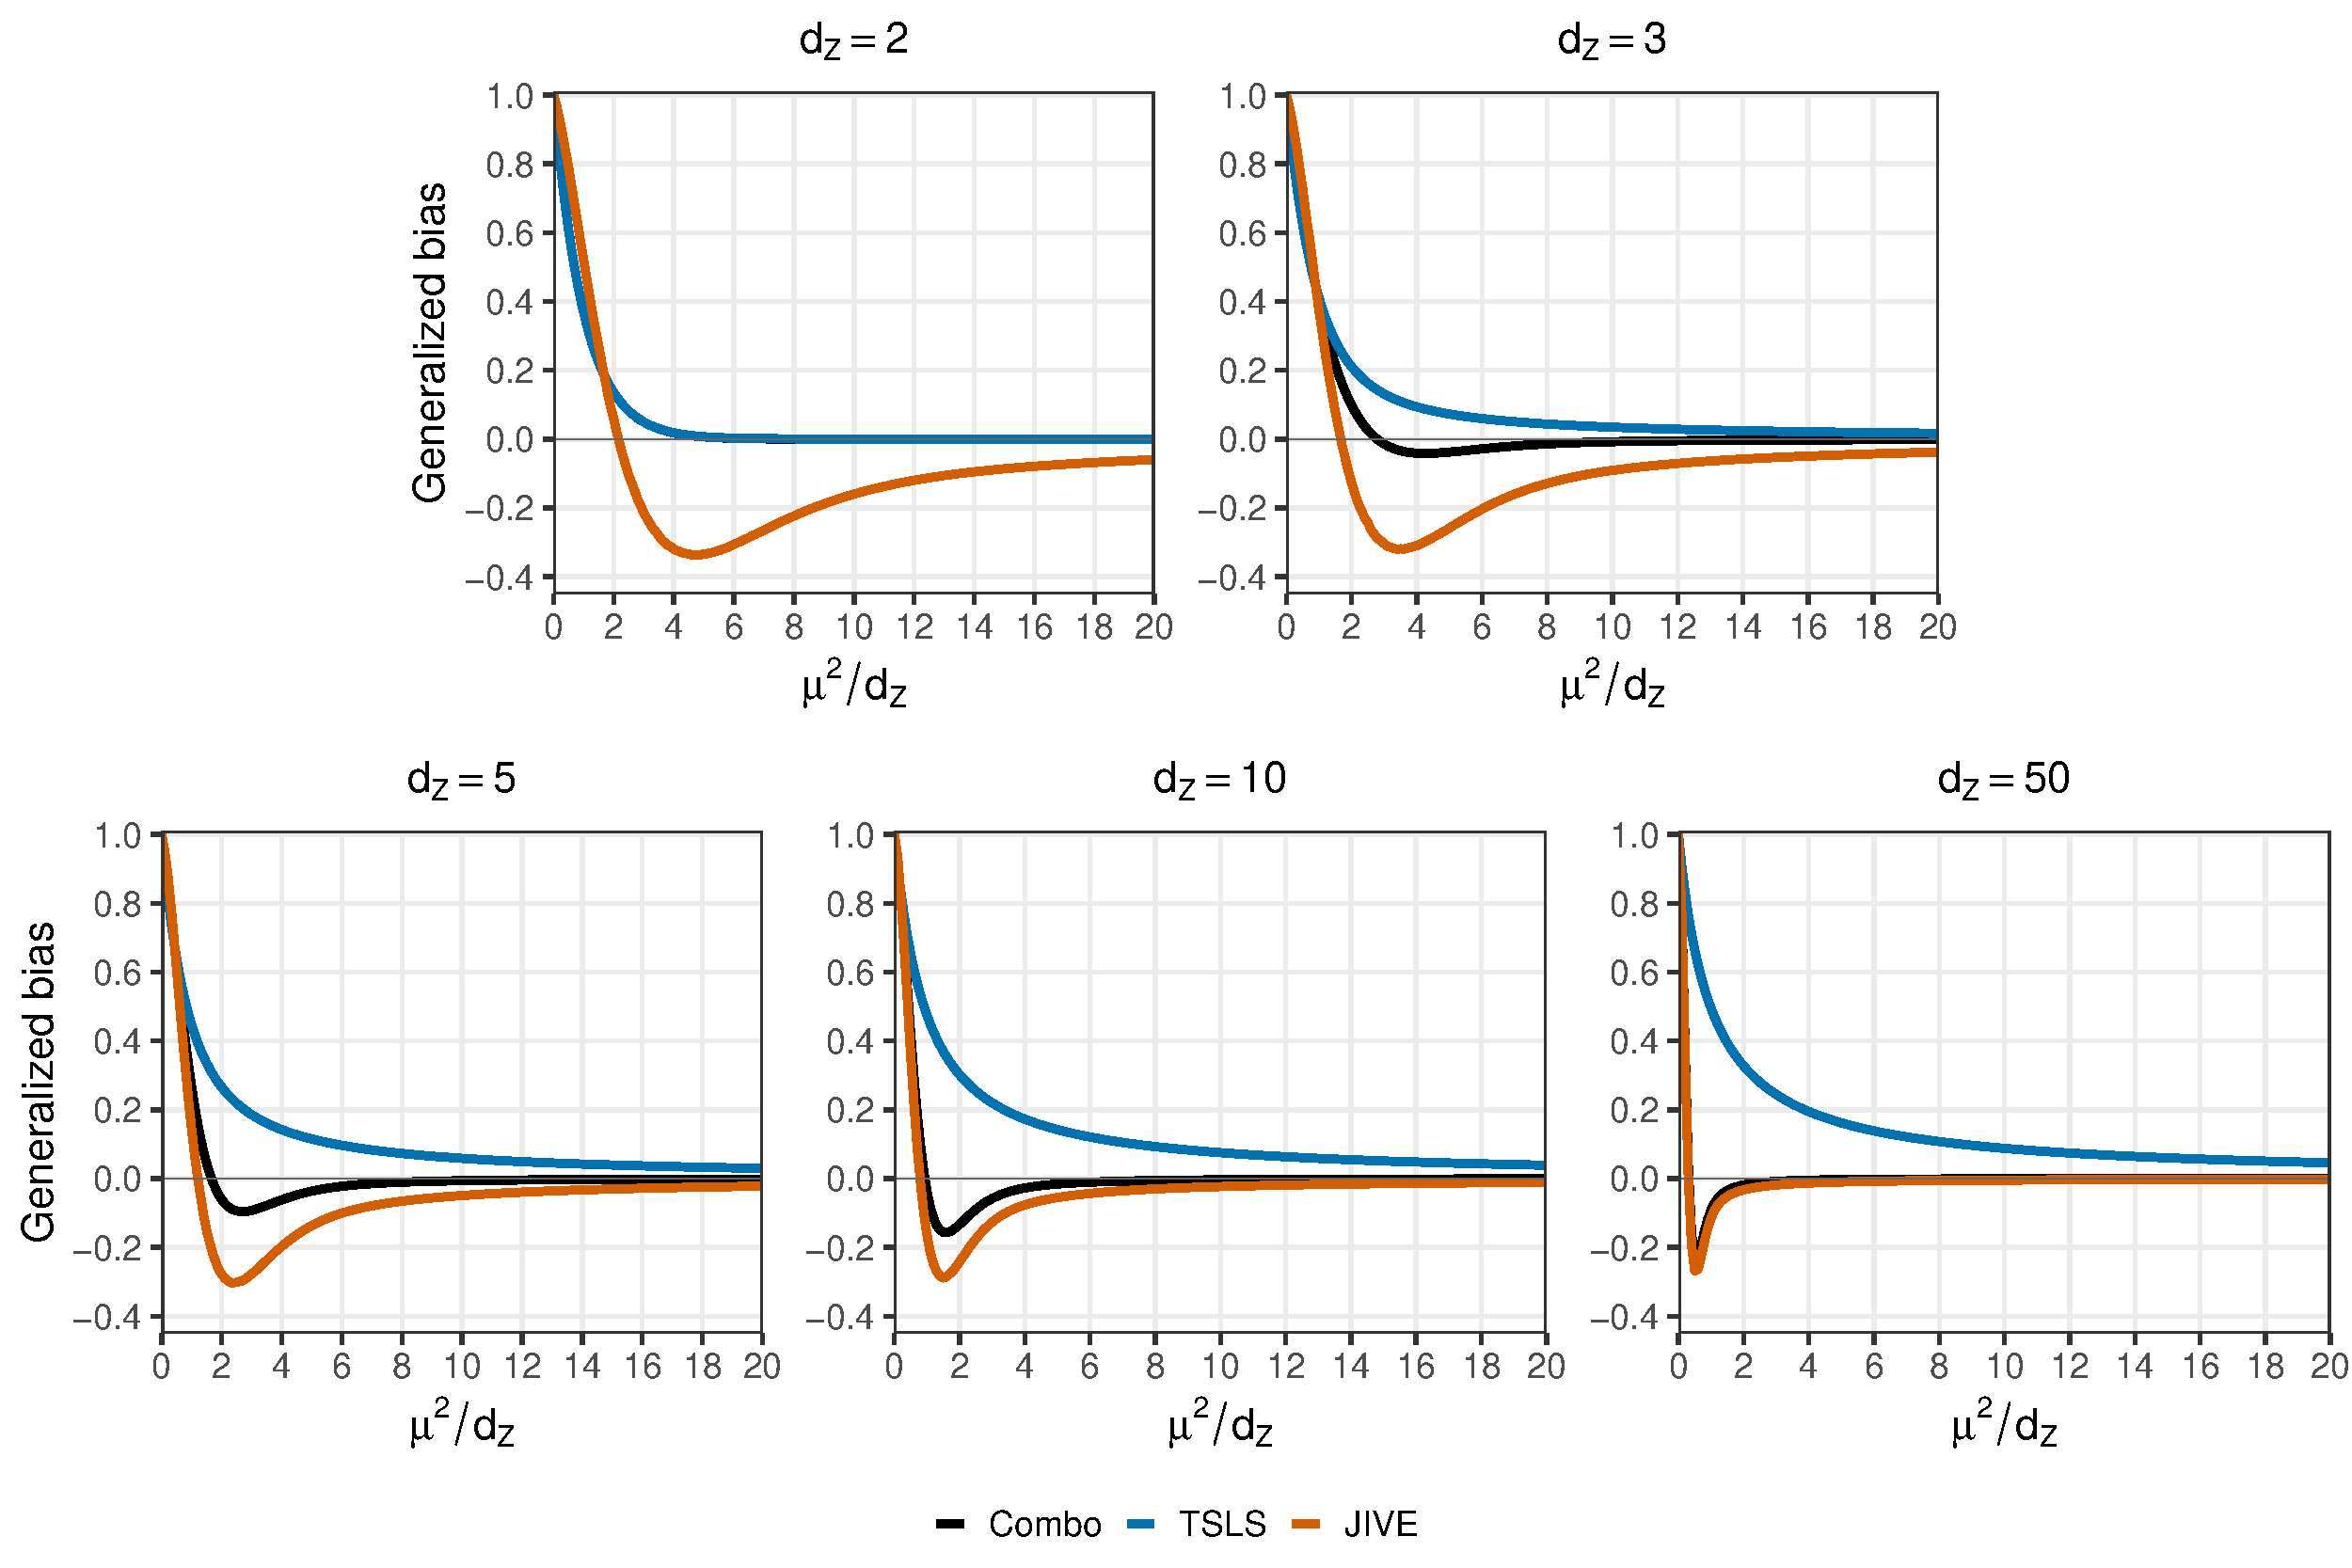
\includegraphics[width=\textwidth]{figs/limit_bias_combo_focus_by_dz.pdf}
%     \caption{\textbf{Generalized Bias of the Combined TSLS-JIVE Estimator.} This figure shows 
%     the generalized bias of the combined TSLS-JIVE estimator for different numbers of instruments, \(d_Z\) and different values of the concentration parameter. Bias is shown as a function of \(\mu^2/d_Z\) which can be thought of as the average concentration of each instrument. The bias of the TSLS and JIVE estimators are shown for comparison. Bias is shown relative to \(\omega\). 
%       }
%     \label{fig:bias-jive-tsls-combined}
% \end{figure}

% It is also of interest to compare it to the estimator that is commonly understood to minimize some notion of bias under the assumption of constant effects, namely the limited information maximum likelihood (LIML) and Fuller-k (\citealp{fullerPropertiesModificationLimited1977}) estimators. These estimators have heteroskedasticity-robust versions (HLIM and HFUL, see \citealp{hausmanInstrumentalVariableEstimation2012}), however these obtain the same limiting distributions as LIML and Fuller-k do under homoskedasticity, hence we focus on these two alternative estimators. We do this in Section \ref{appx:additional-estr-defs} of the \nameref{appx:internet-appendix}.

% \paragraph*{Inference on relative bias.}

% A common way of assessing the bias of the TSLS estimator has been to perform a one-sided test on the composite parameter \(\mu^2/d_Z\), and use this to assess the bias of the estimator relative to the asymptotic bias. This is the approach taken by \cite{stockTestingWeakInstruments2005}, and later \cite{oleaRobustTestWeak2013} in the non-homoskedastic setting. \cite{mogstadBiasIVOne2026} extend this approach to performing two-sided inference on the relative bias of the IV estimator. \cite{mikushevaInferenceManyWeak2022} performs inference on the bias of the JIVE estimator, but only in the regime where \(d_Z \to\infty\). In the following, we extend these approaches to performing inference on relative bias to the weak instruments setting with a fixed number of instruments. We start by recording the limiting distribution  of the first-stage F-statistic along the weak instruments asymptotic sequence.


% \begin{lemmap}{FS}\label{lem:stat-tsls}
% Let \(\hat S_{\hat \gamma}\) be the heteroskedasticity-robust estimator of the asymptotic variance of \(\hat \gamma\). Let
% \(\hat T \equiv \sqrt{n}\,\hat S_{\hat \gamma}^{-\frac{1}{2}}\hat \gamma\), \(\hat F \equiv d_Z^{-1} \lVert\hat T \rVert^2\), 
% Along the weak-instrument asymptotic sequence, when treatment is binary, we have
% \begin{align}
%     \hat T \convd \mu + R \sim \mathfrak{N}(\mu,\boldsymbol{\iota}_{d_Z})
% \end{align}
% and \(d_Z\hat F \convd \mathfrak{C}^2_{d_Z}\).
% \end{lemmap}
% \begin{proof}
%     See Appendix X.
% \end{proof}
% \noindent
% We can use this result to derive bounds on the bias of the TSLS, JIVE and combined TSLS-JIVE estimators. We record this as a proposition.

% \begin{propositionp}{RB}\label{lem:rb-tsls}
%     Let \(\chi_{d_Z,a}^{-1}(d_Z\hat F)\) denote the non-centrality parameter to which \(d_Z\hat F\) corresponds to the \(a^{th}\) quantile of the non-central chi-squared distribution with \(d_Z\) degrees of freedom. Then,
%     \begin{align}
%         % \mu^2 \in 
%         \left[\chi_{d_Z,1-\alpha}^{-1}(d_Z\hat F),\infty\right) \qquad \text{and} \qquad
%         % \mu^2 \in 
%         \left[\chi_{d_Z,1-\frac{\alpha}{2} }^{-1}(d_Z\hat F),\chi_{d_Z,\frac{\alpha}{2} }^{-1}(d_Z\hat F)\right]
%     \end{align}
%     are \(1-\alpha\) confidence intervals for \(\mu^2\).
%     Let \(A(\hat F, \alpha)\) denote such a confidence interval, and let \(\tilde b^{j}_{d_Z}(\mu^2)\) denote the relative bias of the TSLS, JIVE or combined TSLS-JIVE estimator. Then
%     \begin{align}
%         \tilde C(\hat F, \alpha)
%         \equiv \left[\inf_{\mu^2\in A(\hat F, \alpha)} \tilde b_{d_Z}(\mu^2),\sup_{\mu^2\in A(\hat F, \alpha)} \tilde b_{d_Z}(\mu^2)\right]
%     \end{align}
%     is a \(1-\alpha\) confidence interval for the relative bias, and \(\tilde b_0 \notin \tilde C(\hat F, \alpha)\) is a valid test for relative bias at level \(\alpha\).
% \end{propositionp}
% \begin{proof}
%     See Appendix X.
% \end{proof}

% \noindent 
% Having developed a test for the relative bias of the TSLS, JIVE and combined TSLS-JIVE estimators, it is of interesting to understand which first-stage F-statistics reject which amounts of bias of the three estimators. \Cref{tab:inference-bias-estrs}, columns 1--3, tabulate the concentration parameters at which the three estimators have 10\% relative bias. In column 4--6, we tabulate the first-stage F statistic which rejects the hypothesis \(\tilde b > 10\%\), i.e. that the estimator has more than 10\% relative bias. We see that the combined estimator dominates the two other estimators in terms of which \(\hat F\) realization rejects 10\% bias.

% \begin{table}[!htb]
%     \centering
%     \caption{\textbf{Inference on 10\% Relative bias in IV estimators.}}
%     {
%     \renewcommand{\baselinestretch}{1.15}\small
%     \begin{tabularx}{\linewidth}{l>{\centering\arraybackslash}X>{\centering\arraybackslash}X>{\centering\arraybackslash}X>{\centering\arraybackslash}X>{\centering\arraybackslash}X>{\centering\arraybackslash}X}
\toprule
& \multicolumn{3}{c}{Panel A.~$\mu^2\!/d_Z > \bar{\mu}^2\!/d_Z$} & \multicolumn{3}{c}{Panel B.~$\hat{F} > \bar{F}$} \\
\cmidrule(lr){2-4} \cmidrule(lr){5-7}
$d_Z$ & TSLS & JIVE & Combo & TSLS & JIVE & Combo \\
\midrule
2 & 2.30 & 13.60 & 2.30 & 7.9 & 24.1 & 7.9 \\
3 & 3.78 & 9.43 & 1.99 & 9.2 & 16.9 & 6.4 \\
4 & 5.00 & 7.33 & 1.60 & 10.2 & 13.3 & 5.3 \\
5 & 5.78 & 6.05 & 1.34 & 10.8 & 11.1 & 4.6 \\
6 & 6.31 & 5.19 & 2.85 & 11.1 & 9.6 & 6.6 \\
7 & 6.70 & 4.57 & 2.75 & 11.3 & 8.6 & 6.2 \\
8 & 6.98 & 4.10 & 2.62 & 11.4 & 7.8 & 5.9 \\
9 & 7.21 & 3.73 & 2.49 & 11.4 & 7.2 & 5.6 \\
10 & 7.38 & 3.43 & 2.37 & 11.5 & 6.6 & 5.3 \\
15 & 7.92 & 2.51 & 1.92 & 11.5 & 5.1 & 4.3 \\
20 & 8.19 & 2.03 & 1.63 & 11.4 & 4.3 & 3.8 \\
25 & 8.35 & 1.73 & 1.44 & 11.4 & 3.8 & 3.4 \\
30 & 8.46 & 1.52 & 1.30 & 11.3 & 3.4 & 3.1 \\
35 & 8.54 & 1.36 & 1.19 & 11.3 & 3.2 & 2.9 \\
40 & 8.60 & 1.25 & 1.10 & 11.2 & 3.0 & 2.8 \\
45 & 8.64 & 1.15 & 1.03 & 11.2 & 2.8 & 2.7 \\
50 & 8.68 & 1.07 & 0.97 & 11.1 & 2.7 & 2.6 \\
\bottomrule
\end{tabularx}

%     }
%     \begin{flushleft} \vspace{-12pt}
%     {\footnotesize Note: This table shows the first-stage F-statistic cutoffs for the test of 10\% relative bias for three different estimators, the TSLS, JIVE and TSLS-JIVE combined estimator. The first three columns show the normalized concentration parameter, \(\bar\mu^2/d_Z\), at which the estimator has 10\% bias. The last three columns show the first-stage F statistic that rejects the test of more than 10\% relative bias.
%     }    
%     \end{flushleft}
%     \label{tab:inference-bias-estrs}
% \end{table}

% \paragraph*{Inference on absolute bias.}

% \textcolor{red}{TBD. Extend results to binary treatment. Need to figure out the projection stuff, maybe this actually has to be an LR test like the main test with some condition on omega. If so maybe later. }

